\documentclass[12pt,a4paper]{report}
\usepackage[T2A]{fontenc}
\usepackage[utf8]{inputenc}
\usepackage[russian]{babel}
\usepackage{graphicx, setspace}

\usepackage[
top = 1.25cm, 
bottom = 2.0cm]{geometry}

\begin{document}
\begin{titlepage} 
	\centering
    % HEADER
	{
        \scshape
        Федеральное государственное автономное образовательное учреждение высшего образования
        \par
        \textbf{«Научно-образовательная корпорация ИТМО»}
        \par
        \vspace*{1cm}
        Факультет Программной Инженерии и Компьютерной Техники
        \par
    }
    % LOGO
    \vspace*{0.6cm}
    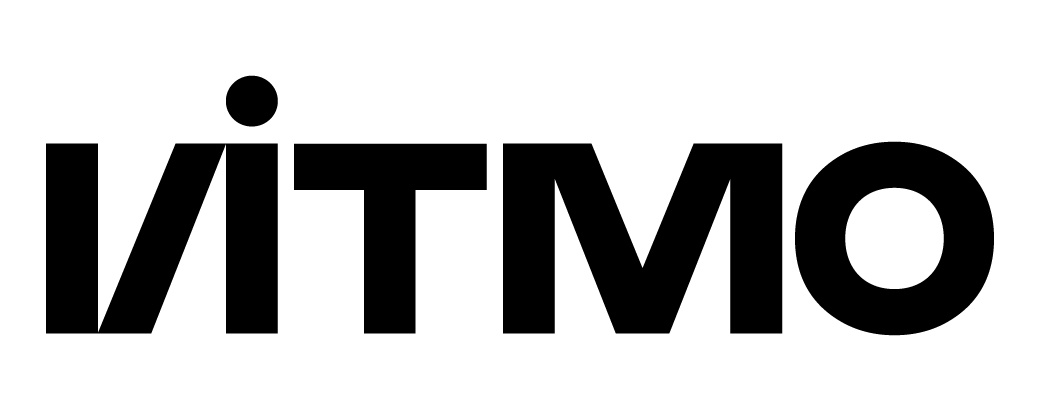
\includegraphics[width=\textwidth]{logo.png}
    % LAB INFO
    {
        \Large
        \textbf{Домашнее задание по теории графов №3}
        \par
        \normalsize
        \vspace*{0.75cm}
        \textbf{Вариант 92}
        \par
    }
    \vfill
    % СREDITS
    \hfill\begin{minipage}{\dimexpr\textwidth-7.8cm}
        \textbf{Выполнил:}\par
        Степанов Арсений Алексеевич\par
        \vspace*{0.15cm}
        \textbf{Группа:}\par
        P3109\par
        \vspace*{0.15cm}
        \textbf{Преподаватель:}\par
        Поляков Владимир Иванович\par
    \end{minipage}
    \vfill
    Санкт-Петербург, \the\year{}г.
\end{titlepage}  
\onehalfspacing
\section*{Матрица смежности графа}
\begin{tabular}{|c|c|c|c|c|c|c|c|c|c|c|c|c|c|}
    \hline
    V/V & $e_{1}$ & $e_{2}$ & $e_{3}$ & $e_{4}$ & $e_{5}$ & $e_{6}$ & $e_{7}$ & $e_{8}$ & $e_{9}$ & $e_{10}$ & $e_{11}$ & $e_{12}$ \\
    \hline
    $e_{1}$  & 0 &   &   & 5 &   &   &   & 4 & 1 & 4 &   & 1 \\
    \hline
    $e_{2}$  &   & 0 &   &   & 4 &   & 4 &   & 1 &   &   &   \\
    \hline
    $e_{3}$  &   &   & 0 & 5 &   & 4 & 3 & 4 &   & 3 & 3 &   \\
    \hline
    $e_{4}$  & 5 &   & 5 & 0 &   &   & 1 &   &   &   &   & 1 \\
    \hline
    $e_{5}$  &   & 4 &   &   & 0 & 4 & 4 &   &   &   &   & 5 \\
    \hline
    $e_{6}$  &   &   & 4 &   & 4 & 0 & 5 &   & 3 &   &   & 2 \\
    \hline
    $e_{7}$  &   & 4 & 3 & 1 & 4 & 5 & 0 & 2 &   &   & 5 &   \\
    \hline
    $e_{8}$  & 4 &   & 4 &   &   &   & 2 & 0 &   &   & 1 &   \\
    \hline
    $e_{9}$  & 1 & 1 &   &   &   & 3 &   &   & 0 & 4 & 4 &   \\
    \hline
    $e_{10}$ & 4 &   & 3 &   &   &   &   &   & 4 & 0 & 5 & 5 \\
    \hline
    $e_{11}$ &   &   & 3 &   &   &   & 5 & 1 & 4 & 5 & 0 & 2 \\
    \hline
    $e_{12}$ & 1 &   &   & 1 & 5 & 2 &   &   &   & 5 & 2 & 0 \\
    \hline
\end{tabular}
\section*{Рисунок исходного графа}
\begin{center}
    \includegraphics*[width=10cm]{graph_1.png}
\end{center}
\newpage
\section*{Задание}
Небходимо найти путь с максимальной пропускной способностью
\hfill\break
Проводим разрез графа $K_1$:\\
$Q_1=\max(q_{ij})=5$\\
Закорачиваем все рёбра графа, такие что $g_{ij} \leq Q_1$, то есть рёбра\\
$(1, 4)$, $(3, 4)$, $(5, 12)$, $(6, 7)$, $(7, 11)$, $(10, 11)$ и $(10, 12)$\\
Получаем следующий граф:\\
\begin{center}
    \includegraphics*[width=10cm]{graph_2.png}
\end{center}
Проводим разрез графа $K_2$:\\
$Q_2=\max(q_{ij})=4$\\
Закорачиваем все рёбра графа, такие что $g_{ij} \leq Q_2$, то есть рёбра\\
$((1, 3, 4), 8)$, $((1, 3, 4), (5, 6, 7, 10, 11, 12))$, $(2, (5, 6, 7, 10, 11, 12))$ и $(9, (5, 6, 7, 10, 11, 12))$\\
Получаем следующий граф:\\
\begin{center}
    \includegraphics*[width=5cm]{graph_3.png}
\end{center}
\pagebreak
Вершины объединены, полученная пропускная спобность пути $Q(P)=4$,\\
Построим граф, вершины которого являются вершинами исходного графа, 
а рёбра имеют пропускную способность $q_{ij}\geq Q(P)$\\
Получаем следующий граф:\\
\begin{center}
    \includegraphics*[width=10cm]{graph_4.png}
\end{center}
Таким образом получаем, что пропускная способность пути от вершины $e_1$ до вершины $e_{12}$ равна 4
\end{document}
